\chapter{Data and Cohort Description}

This chapter describes the clinical and imaging-derived dataset used throughout this project,
the selection criteria applied to obtain the analysis cohort, and the data structures available
for each patient case. All cases originate from the DEVELOP registry, a prospective
collection of post-myocardial infarction patients studied at Centro M\'{e}dico Teknon (Barcelona,
Spain) in the context of ventricular tachycardia (VT) risk assessment.

\section{The DEVELOP Registry and Clinical Context}

The source data consist of anonymised late gadolinium enhancement cardiac magnetic
resonance (LGE-CMR) studies from the DEVELOP registry. The original DICOM acquisitions
are stored in Teknon's internal storage system. The working dataset used in this project does
not operate directly on the DICOM files; instead, it uses the three-dimensional anatomical
and tissue meshes exported after post-processing. The dataset spans five acquisition years
(2021--2025), and the internal folder organisation within each year reflects the evolution of
the ADAS 3D export pipeline over time.

For each patient, image post-processing was carried out using ADAS 3D (Galgo Medical,
Barcelona), a software platform for three-dimensional cardiac image analysis. ADAS 3D
reconstructs the left ventricular (LV) shell from the LGE-CMR study and performs
semi-automatic tissue characterisation based on signal intensity. The software distinguishes
dense scar (core zone, CZ), heterogeneous peri-infarct tissue (border zone, BZ), and
healthy myocardium. The resulting surfaces are exported as VTK meshes, which constitute
the primary geometric input to the analyses in this work.

\section{Data Acquisition and Processing at Teknon}

Data extraction was performed on-site at Centro M\'{e}dico Teknon's computer system.
Building on prior familiarity with ADAS 3D acquired before the collaboration, the
understanding of the segmentation workflow was substantially deepened through direct
interaction with Teknon's technicians and clinicians: how scar appears under different
acquisition conditions, how tissue thresholds are adjusted, and how the resulting 3D models
relate to the underlying cardiac anatomy. Beyond the left ventricle, this experience also
provided exposure to left atrial ablation workflows and different arrhythmia types, including
atrial fibrillation and typical and atypical flutter.

Since no automatic pipeline existed for batch retrieval of specific mesh files from the ADAS
3D exports, a one-by-one extraction of CZ, BZ, healthy tissue, and corridor files was
undertaken for each patient. Version inconsistencies in file naming across acquisition years
(different ADAS 3D versions exported under DE-MRI, DE-MRI 3D, or DE-MRI 2D labels, and
the spelling variant TRANSMURABILITY for TRANSMURALITY) required the automated
loader to use pattern-based search rather than exact filenames.

The local dataset is organised as \texttt{/Basal/Data/LV/}. The automated scanner resolves
DE-MRI variants in order, locates anatomical meshes (Endo Layer, Epi Layer, Left
Ventricle, Myocardium), and searches the \texttt{LV/TISSUE/} subdirectory using ordered
glob patterns for core zone, border zone, healthy, scar, layer, and corridor files.

\section{Cohort Selection and Exclusion Criteria}

A case was considered valid only if it contained both a valid LV reconstruction directory and
a core zone mesh found inside \texttt{LV/TISSUE/}. An automated scan of the dataset was
performed across all patient folders.

Of the 168 total patient folders, 118 (70.2\%) contained a valid LV reconstruction directory,
and 105 (62.5\%) additionally contained a CZ mesh (Table~\ref{tab:cohort}). These 105
cases constitute the valid cohort. The 63 excluded cases fall into two categories: 50 lacked
an LV reconstruction directory entirely (35 had a \texttt{Basal/Data} path but no recognised
DE-MRI folder; 15 had no \texttt{Basal/Data} path), and 13 had an LV reconstruction but no
usable CZ mesh. The patient-level list of excluded cases is provided in Annex~\ref{app:supplementary}.

All 105 valid cases are used in the analyses presented in this work. No held-out split was
applied, as the primary objective is to build and evaluate a geometric representation rather
than to train a predictive model.

\begin{table}[htbp]
    \centering
    \caption{Cohort selection summary.}
    \label{tab:cohort}
    \begin{tabular}{lrr}
        \toprule
        Category & $n$ & \% \\
        \midrule
        Total patient folders & 168 & 100.0 \\
        With valid LV reconstruction & 118 & 70.2 \\
        With valid CZ mesh (analysis cohort) & 105 & 62.5 \\
        \midrule
        Excluded: no LV reconstruction directory & 50 & 29.8 \\
        \quad of which: Basal/Data present, no DE-MRI folder & 35 & --- \\
        \quad of which: no Basal/Data path & 15 & --- \\
        Excluded: LV present, no usable CZ mesh & 13 & 7.7 \\
        \bottomrule
    \end{tabular}
\end{table}

\section{Available Data per Patient}

Each valid case provides: (i) LV shell meshes representing the endocardial and epicardial
boundaries; (ii) tissue classification surfaces from ADAS 3D, primarily the core zone, with
additional border zone, healthy, and corridor meshes when available; (iii) transmural layer
meshes (Layer\_10 through Layer\_90), representing concentric wall-depth levels at 10\%
increments from the endocardial surface; and (iv) clinical metadata from the DEVELOP
registry CSV, including demographics, MRI-derived scar metrics, echocardiography,
arrhythmia variables, and follow-up outcomes. A detailed description of the clinical metadata fields and their completeness is provided in
Annex~\ref{app:supplementary}. The registry CSV is severely sparse outside MRI-derived
scar metrics: while LV mass, core zone, and border zone variables are available for
$\geq$96\% of registry entries, most demographic and clinical variables fall below 55\%
completeness, and outcome variables (dates of death, ablation, device implant) are available
for fewer than 6\% of entries. Sex information was available for 48 of the 105 valid patients,
with a predominantly male distribution consistent with the epidemiology of myocardial
infarction. Age was available for a subset of 48 patients (mean $63.0 \pm 11.5$ years). This
degree of missingness makes supervised clinical outcome modelling infeasible at the current
scale and motivates the use of the full cohort without clinical sub-grouping.

\section{Quality Control}

An automated three-dimensional rendering pipeline was implemented using PyVista. For
each case, the LV shell is displayed as a semi-transparent surface with the core zone
overlaid in opaque red from an isometric viewpoint. The resulting thumbnails were
assembled into a per-patient grid, enabling rapid visual inspection of segmentation
consistency, scar extent, and anatomical plausibility. This quality control step confirmed that
the 105 valid cases produce geometrically coherent scar representations suitable for
downstream analysis.

\begin{figure}[htbp]
    \centering
    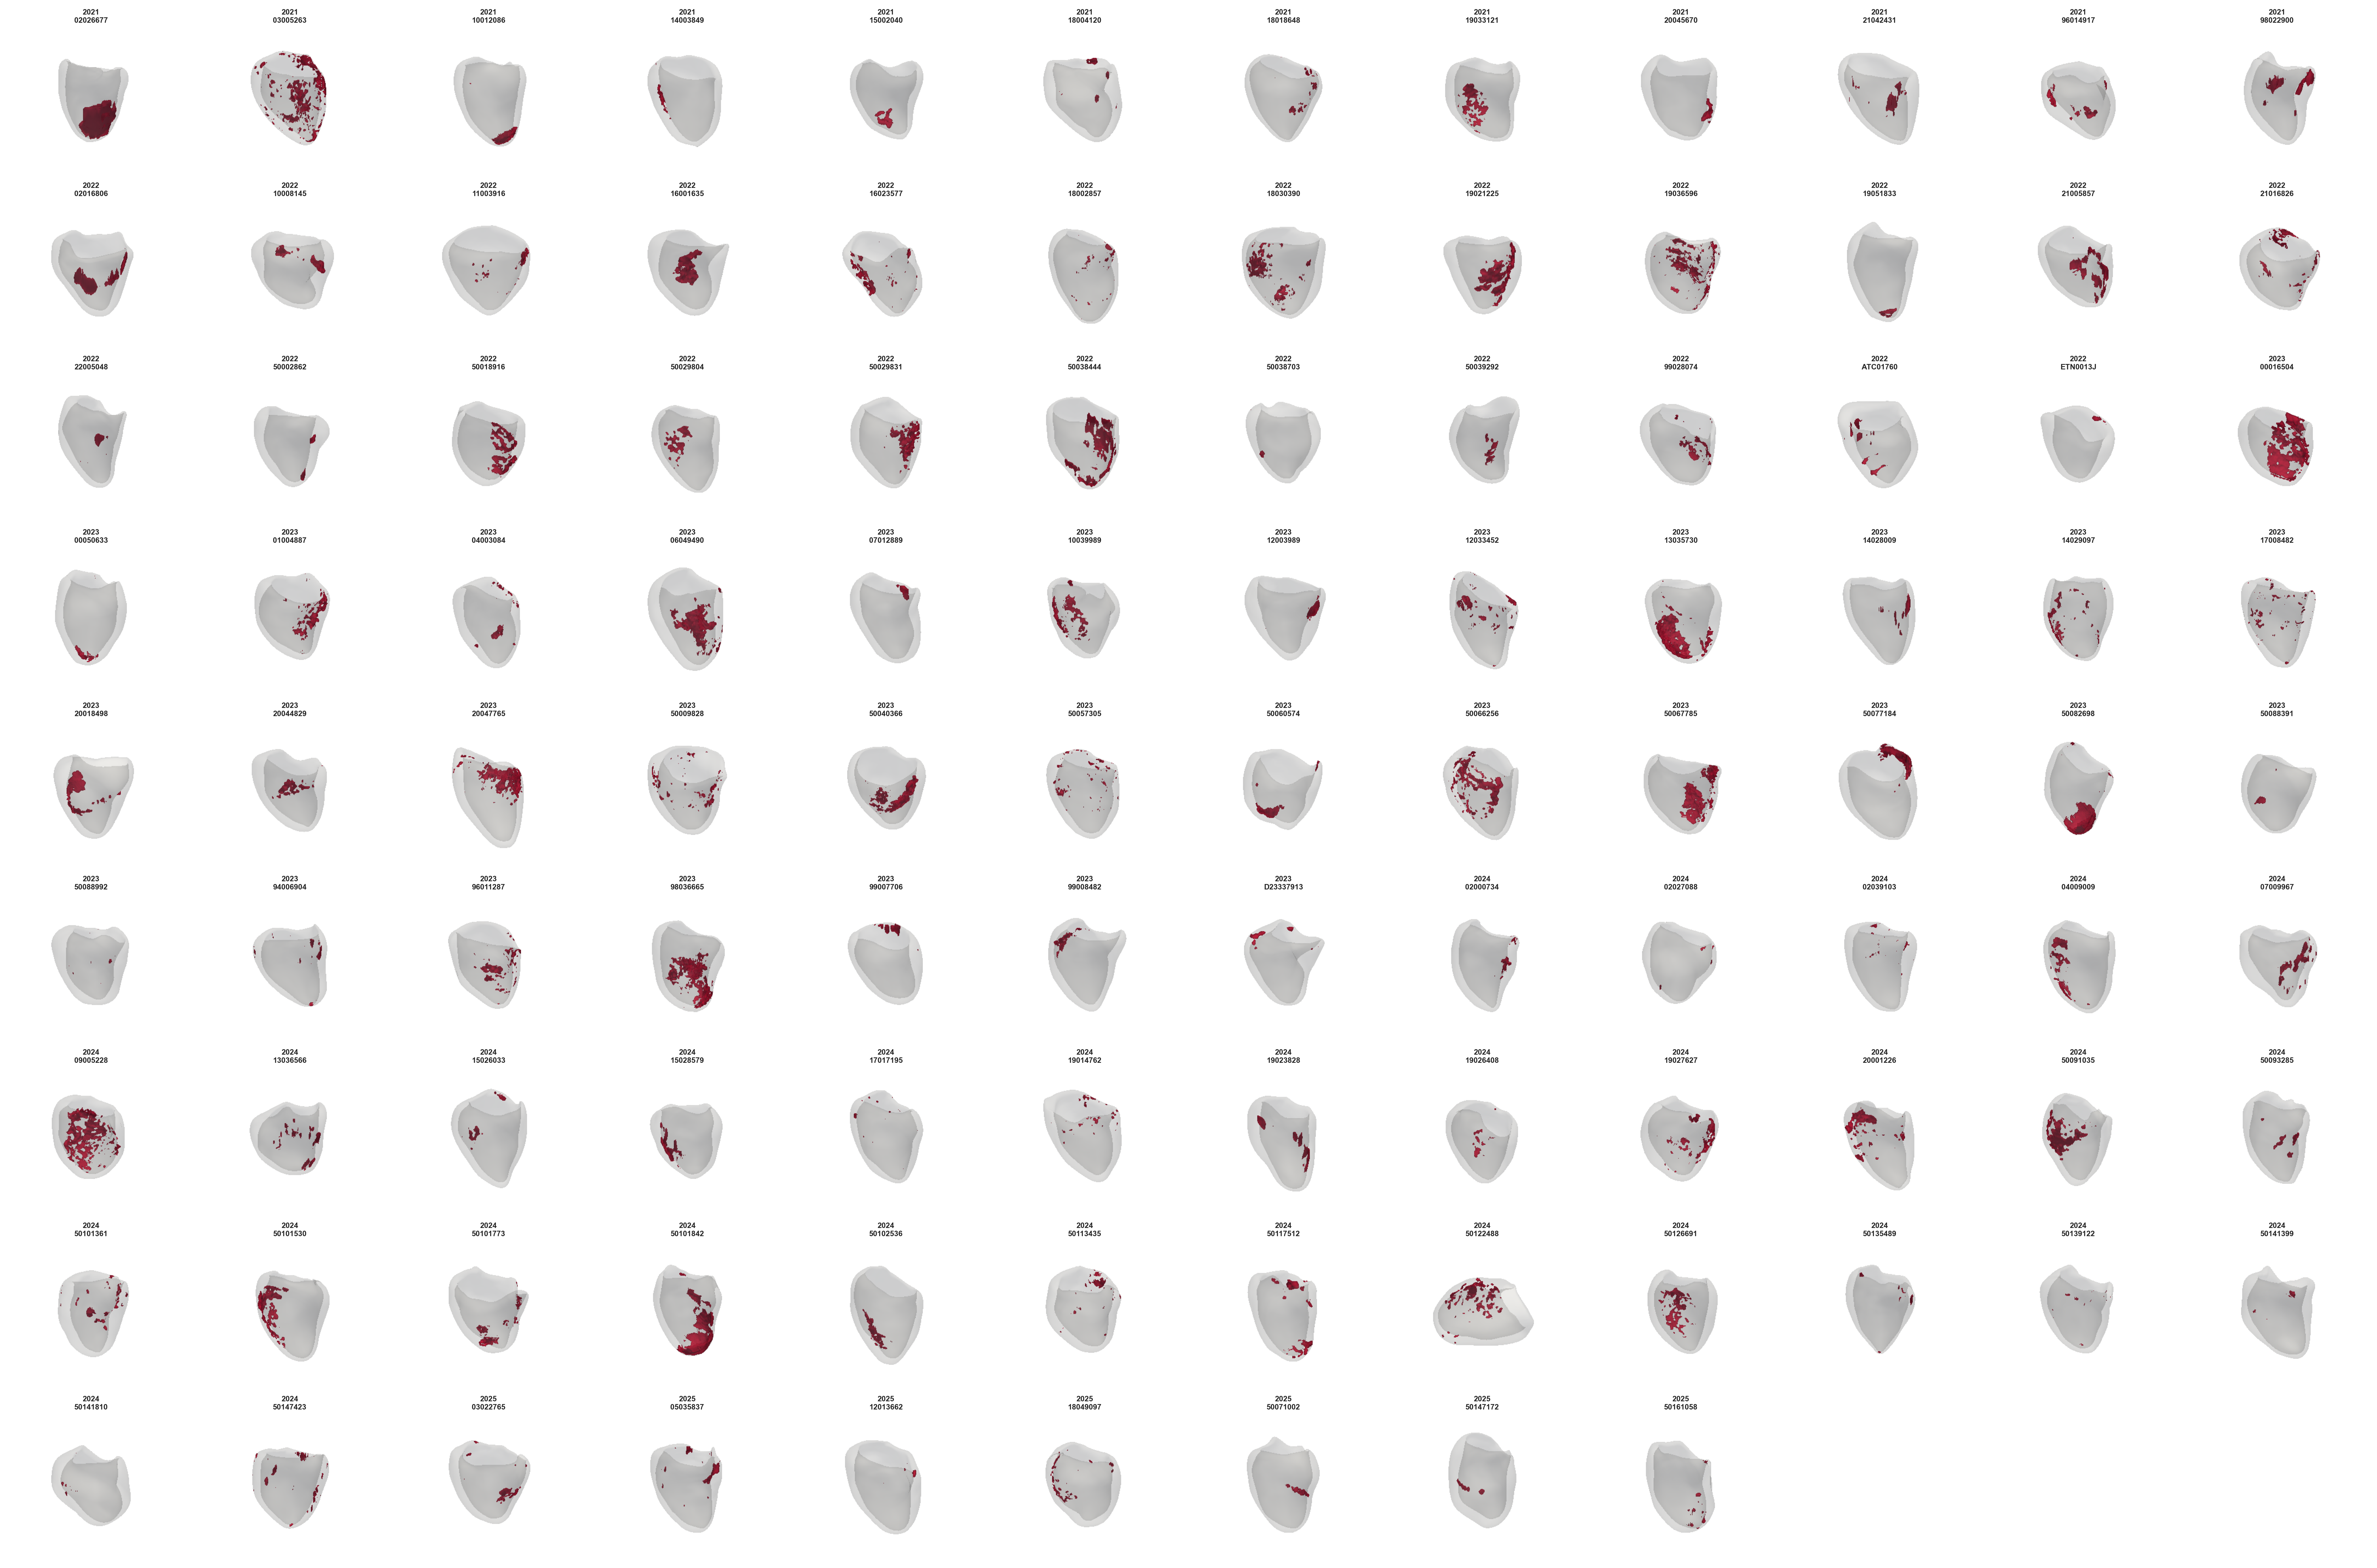
\includegraphics[width=\textwidth]{figures/3d_grid_full_cohort}
    \caption{QC grid of all 105 cases: LV shell (semi-transparent) with core-zone scar (red). Illustrates the cohort's wide range of scar extent, location, and morphology.}
    \label{fig:qc_grid}
\end{figure}
